\subsection{Overview}
The DSL is divided into three components, a arithmetic expressions language, a language for specifying a web site and a language for specifying input sources for the system. 
The expression language is a utility language which is included by the two others. 
This language defines how a user can create arithmetic expressions in either of the other two languages. 
The Web visualizer is a language to create dynamic web sites, like the sample page shown on the front page. 
This language lets the user create pages on a site, link different pages to each other and visualize information through the use of graphs. 
The Datasources language, which is still to be developed, will be used to specify different data sources, like for instance a external databases or APIs. 
In addition this language will also be used to specify internal persistence and a API for other systems to use for posting data to the Dashk system.

\subsection{The Formula Expression Language}
The Formula Expressions DSL is responsible for understanding mathematical formulas, which will be applied to tables of data.
\paragraph{Meta model}
The formula metamodel consist of multiple elements.
The types include in the elements included in the model are:
\begin{enumerate}
\item Formula: The overall Structure Element
\item Variable: The varaible names included in the formula
\item Expression: The right side of the equal sign in $f(x) = x \cdot x$. The Expression collects the parts which is connected with plus($+$) and minus($-$). 
\item Factor: A semi-structure of the expression, Factors collects the parts connected with multiplication($\cdot$) and division($/$).
\item Op1: Identifies a addition or substraction operation
\item Op2 Identifies a multiplication or divison a operation
\item Primitiv: Identifies as either a number or a Variable
\end{enumerate}

\begin{figure}
  \begin{center}
    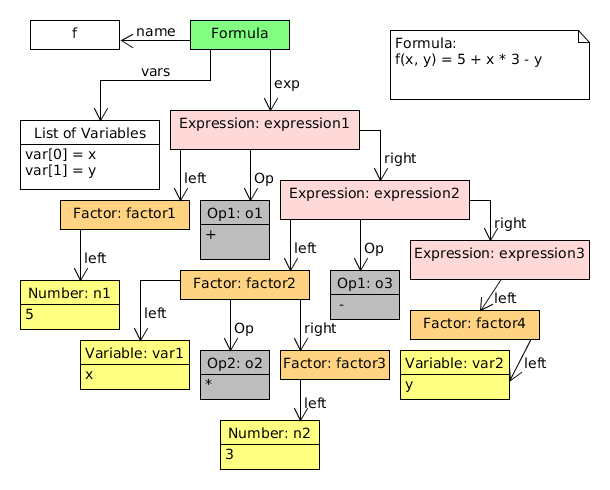
\includegraphics[width=\linewidth]{images/formulaInstance}
  \end{center}
  \caption{Instance of Formula}
  \label{fig:formulaInstance}
\end{figure}
    

Given the following the example: $$f(x, y) = 5 + x \cdot 3 - y$$
The rules for the grammar is explained as below also referring to Figure \ref{fig:formulaInstance}:
\\
A Formula Contains a name which is defined a the letter/word in front of the paranthesis
also underlined in the following formula: $\underline{f}(x, y) = 5 + x \cdot 3 - y$.
It also contains a list of variables, defined within the paranthesis seperated
by ``,'' as underlined: $f\underline{(x, y)} = 5 + x \cdot 3 - y$. Finally the expression
of the formula is everything on the right side of the equal-sign(``=''), here follows
the rule that every variable used in the expression has to appear inside the paranthesis
of the formula as well, as it works as a function, the expression part underlined:
$f(x, y) = \underline{5 + x \cdot 3 - y}$.

Looking at the expression: $5 + x \cdot 3 - y$ it is broken down by taking continouisly
working from the left to the right, from the expression perspective by taking one factor
at a time. For the Expression the factors for the expression is $5$, $x \cdot 3$ and $y$
as underlined: $\underline{5} + \underline{x \cdot 3} - \underline{y}$. Once a factor
is found. the rest of the expression is defined as a new expression which is the right
side to the Expression.
At first the expression would contain the factor $5$ and the of the expression would be
a nested expression for the overall expression.

\begin{figure}
  \begin{center}
  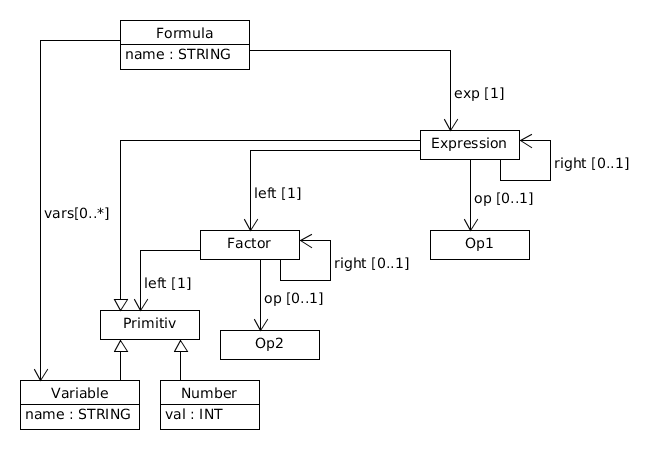
\includegraphics[width=\linewidth]{images/MetaFormula}
  \end{center}
  \caption{Model of the formula module}
  \label{fig:formulaModel}
\end{figure}
\paragraph{Code Generation}

\subsection{The Web visualizer Language}
Below table shows the grammar for the web visualizer language to the left and an example of use on the right. 
As seen from the left side the system consist of a number of pages which again consists of a number of tiles. 
One tile can, in current implementation be either a link to another page or a definition of a graph. 
Since the datasource language have not yet been implemented the web visualizer language currently work with a hard-coded testset. 
Further are only one graph type implemented (a line chart), however the system makes use of D3 framework meaning that extending the system with other graph types is a smaller task.

%Some table

The example on the right site creates a System instance with three pages, each page with a number of Links and Graphs.

\paragraph{Meta model}
Below is the first meta model of the system. 
This model matches the language specification one to one. 
The System once again is a collection of pages, which again consists of a number of tiles which can be of the two previous described types. 

\begin{figure}
\begin{center}
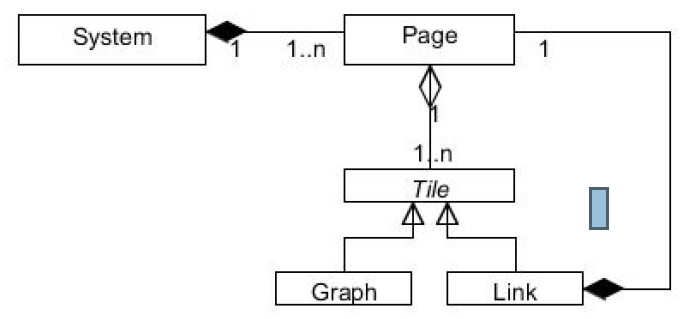
\includegraphics[width=\linewidth]{images/websitelanguagemodel}
\end{center}
\caption{Model of the language}
\label{fig:websitelangmodel}
\end{figure}

\paragraph{Code generation}
To create the website the project uses the Django framework. 
This framework uses an MVC architektur which is extended with a template pattern with HTML documents. 
In order to make the output easy readable and customizable for a user, the first meta model needs to be mapped to a second meta model with more explicit information which matches the MVC architecture better.
This second model can be seen in below diagram. 

\begin{figure}
\begin{center}
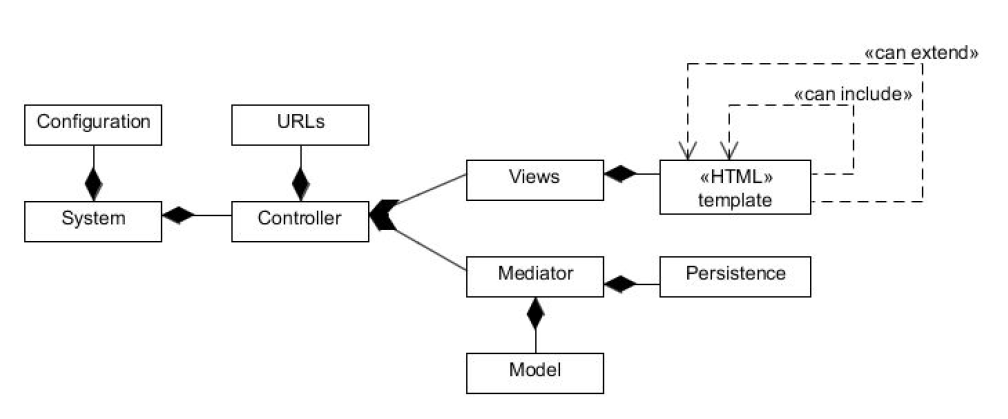
\includegraphics[width=\linewidth]{images/websitemodel}
\end{center}
\caption{Model of the Website}
\label{fig:websitemodel}
\end{figure}


The first step of mapping the previous model into the second meta model, is to create a system with a configuration. 
Secondly a default controller is added with the default Django Admin configuration pages. 
This controller gets a number of URLs and default views. 
After this a second controller gets added, this controller is used for the pages defined in the language. 
Each page gets transformed into a url entity, view entity, model and a template HTML-file.
The HTML file holds a easy customizable structure of the content added to the page. The view and model will in time be connected to the Data sources from the previous specified language. 
In addition will the view of a page be responsible of rendering the template with context and data from a datasource. 
After this model have been created each entry in the model is looped through and generated into a file.

